\section{Motivation}
Buildings consume a large fraction of the energy produced in the United States, and much of it
is wasted\cite{epa}.  They are notoriously complex and although many commercial 
buildings are equiped with a rich sensing infrastructure, ad-hoc data management practices
make it difficult for any analytical solution to be widely ported across building
systems.  For example, consider the following stream names: \texttt{BLDA1R435\_\_ART,
BLDA1R435\_\_ARS, BLDA1R545\_\_ART}. Each name encodes contextual information in the form
of concatinated character sequences. In these, the first 4 characters refer to the 
name of the building, the next one encodes the air handling unit association, the next 
four encode the room,
and the last three encode the acronym for the type.  Although the examples given are well
structured, many variants within the same data set exist.  For example, \texttt{BLD\_1R435\_ARG\_}
is the encoding for a different sensor in the same room as the others, but with a name
that is \emph{like} although not exactly the same structure as the others.

For building engineers this is usually not a problem.  Upon visual inspection, the two
encodings are similar enough that the engineer can decode the meaning.  However, for automatic 
processing, these kinds of variations makes it difficult to generalize the character-contruction
rule set.  Without rule-set construction the data cannot be ingested properly or interpretted
correctly.  However, there are ``active learning'' techniques in the literature~\cite{ms} 
that address this problem by leveraging the knowledge of an expert. The idea behind active learning
is that you can generalize the set of rules that generate a name/tag by example, iteratively
updating the name construction rule set for different types of names.  An expert feeds
the system examples of names for a particular type of sensor, and the algorithms generalize the
character-set construction rules.
We explore the use
of \emph{active learning} techniques to iteratively learn all the variants within an across
data sets.

% walk through an example of point names from 2 or three buildings and explain 
% what's challenging here
%
% BLDA1R435__ART
% BLDA1R435__ARS
% BLDA1R545__ART

% Discuss how active learning technique can be used to "unify" these tag names

% Now discuss how the actual shapes of the readings can be quite similar looking

\begin{figure}[h!]
\centering
    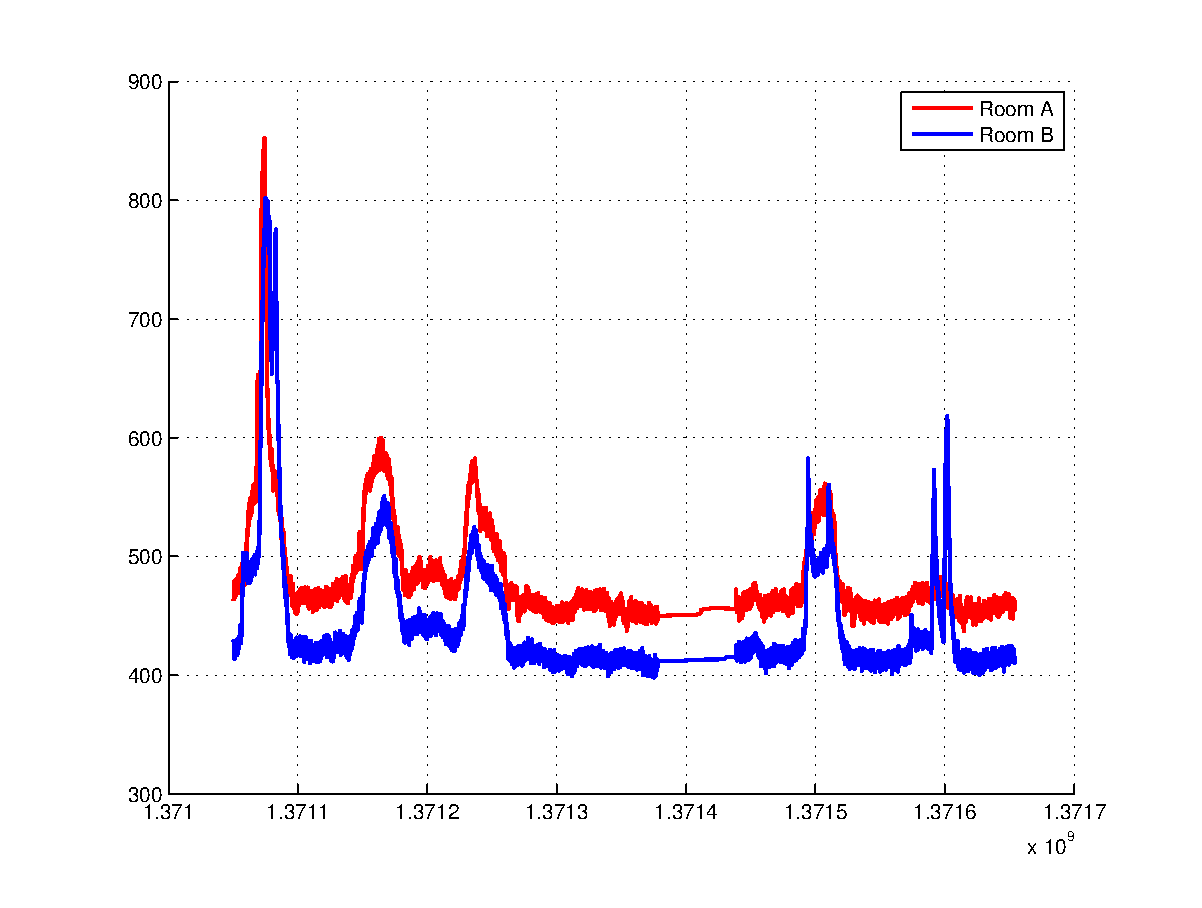
\includegraphics[width=0.48\textwidth]{figs/co2_pair.eps}
    \caption{CO2 sensor traces.}
\label{fig:co2traces}
\end{figure}

\begin{figure}[h!]
\centering
    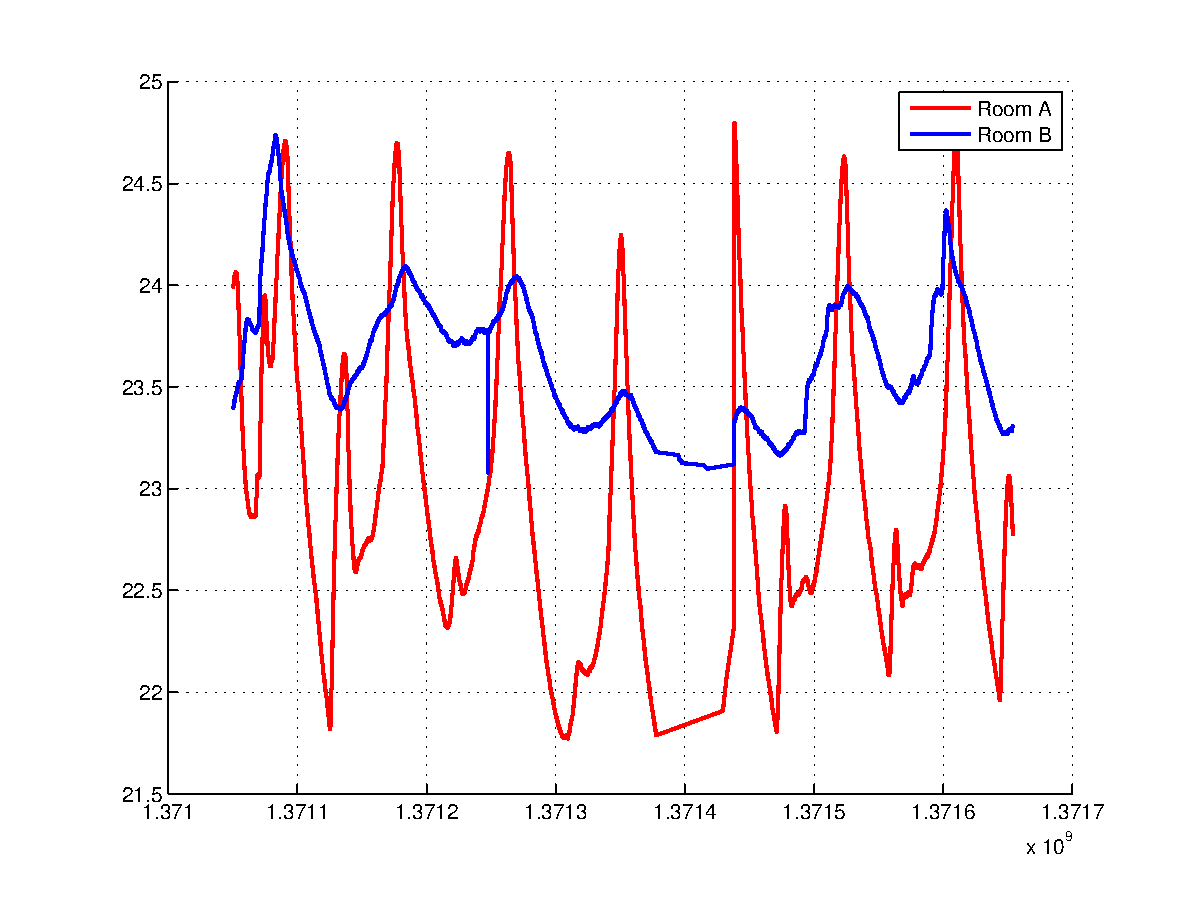
\includegraphics[width=0.48\textwidth]{figs/temp_pair.eps}
    \caption{temperature traces.}
\label{fig:temptraces}
\end{figure}

% tie this into search; search is done for scale
% scale is necessary for broad impact
% 

% discuss how both can be used to generate more metadata that we can use for indexing
